\documentclass{article}
\usepackage[margin=1in]{geometry}
\usepackage{amsmath,amsthm,amssymb}
\usepackage{bbm,enumerate,mathtools}
\usepackage{tikz,pgfplots}
\usepackage{chessboard}
\usepackage[hidelinks]{hyperref}
\usepackage{multicol} % Problem 35
\usepackage{xstring} % Difficulty command
\usetikzlibrary{shapes.geometric}

\newenvironment{question}{\begin{trivlist}\item[\textbf{Question.}]}{\end{trivlist}}
\newenvironment{note}{\begin{trivlist}\item[\textbf{Note.}]}{\end{trivlist}}
\newenvironment{references}{\begin{trivlist}\item[\textbf{References.}]}{\end{trivlist}}
\newenvironment{related}{\begin{trivlist}\item[\textbf{Related.}]\end{trivlist}\begin{enumerate}}{\end{enumerate}}

\newcommand\score[1]{
\pgfmathsetmacro\pgfxa{#1+1}
\tikzstyle{scorestars}=[
  star,
  star points=5,
  star point ratio=2.25,
  draw,
  inner sep=3pt,
  anchor=outer point 5
]
  \begin{tikzpicture}[baseline]
    \draw[opacity=0] (0,-0.5) rectangle (0,0.2); % Workaround for whitespace at the bottom.
    \foreach \i in {1,...,4} {
      \pgfmathparse{(\i<=#1?"yellow":"gray")}
      \edef\starcolor{\pgfmathresult}
      \draw (\i*4.5ex,0) node[name=star\i,scorestars,fill=\starcolor]  {};
    }
  \end{tikzpicture}
}

\newcommand{\difficulty}[1]{%
  \IfEqCase{#1}{%
      {1}{
        
\begin{tikzpicture}[scale=0.7, baseline=0.9mm]%
          \definecolor{slopegreen}{rgb}{0.0, 0.5, 0.0}%
          \fill[slopegreen] (0.5,0.5) circle (0.5);%
        \end{tikzpicture}%
      }%
      {2}{
        
\begin{tikzpicture}[scale=0.7, baseline=0.9mm]%
          \definecolor{slopeblue}{rgb}{0.0, 0.44, 1.00}
          \fill[slopeblue] (0,0) rectangle (1,1);%
        \end{tikzpicture}%
      }%
      {3}{
\begin{tikzpicture}[scale=0.7, baseline=0.9mm]\fill (0,0.5)--(0.5, 0)--(1,0.5)--(0.5,1)--cycle; \end{tikzpicture}}%
      {4}{
\begin{tikzpicture}[scale=0.7, baseline=0.9mm]\fill (0.25,0)--(0,0.5)--(0.25,1)--(0.5,0.5)--cycle; \fill (0.75,0)--(0.5,0.5)--(0.75,1)--(1,0.5)--cycle;\end{tikzpicture}}%
      % you can add more cases here as desired
  }[\PackageError{difficulty}{Undefined difficulty level: #1}{}]%
}%
\newcommand{\rating}[2]{\difficulty{#1}\\\score{#2}\\}


\begin{document}
\rating{2}{1}
The number of ways to draw a triangle on a triangular grid is given by \[
  \sum_{k=1}^{n-1} k\cdot t(n-k)
  = \binom{n+2}{4}
  = A000332(n-2)
\] where $t(m)$ is the $m$-th triangular number, and
\href{https://oeis.org/A000332}{A000332} is a figurate number based on the 4-simplex.

~

\noindent
The number of ways to draw a square on a square grid is given by \[
  \sum_{k=1}^{n-1} k\cdot (n-k)^2
  = \frac 16 \binom{n^2}{2}
  = n^2\left(\frac{n^2 - 1}{12}\right)
  = A002415(n)
\] where \href{https://oeis.org/A002415}{A002415} is a figurate number based on the 4-dimensional pyramid.

~

\noindent
The number of ways to draw a hexagon on a hexagonal grid is given by \[
  \sum_{k=1}^{n-1} k\cdot h(n-k)
  = n\binom {n+2}3
  = \frac{n^2(n+1)(n+2)}{6}
  = A002417(n-1).
  % = \sum_{k=1}^{n-1} k^3 = t(n-1)^2
\] where $h(m)$ is the $m$-th hexagonal number, and \href{https://oeis.org/A002417}{A002417} is a 4-dimensional figurate number.
\begin{figure}[ht!]
  \centering
  % Triangle
  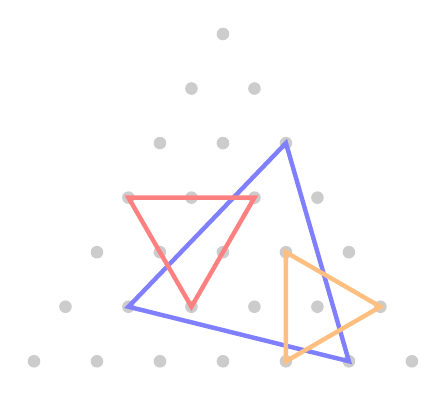
\begin{tikzpicture}[scale=0.8]
    \foreach \x in {1,...,7} {
      \foreach \y in {1,...,\x} {
        \fill[gray!40] ({\x - \y/2}, {sqrt(3)/2 * \y}) circle (0.1);
      }
    }
    \draw[ultra thick, blue!50] (2, {sqrt(3)})--(4.5, {5/2*sqrt(3)})--(5.5, {sqrt(3)/2})--cycle;
    \draw[ultra thick, red!50] (3, {sqrt(3)})--(4, {4/2*sqrt(3)})--(2, {4/2*sqrt(3)})--cycle;
    \draw[ultra thick, orange!50] (4.5, {sqrt(3)/2})--(4.5, {3/2*sqrt(3)})--(6, {sqrt(3)})--cycle;
  \end{tikzpicture}
  \hspace{0.7cm}
  % Square
  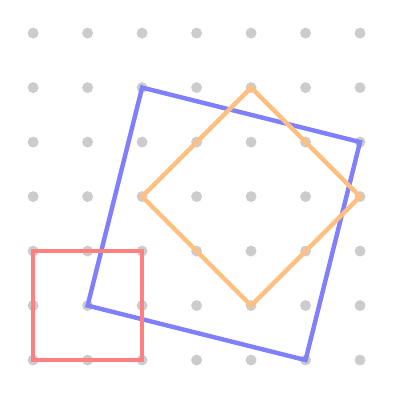
\begin{tikzpicture}[scale=0.692]
    \foreach \x in {1,...,7} {
      \foreach \y in {1,...,7} {
        \fill[gray!40] (\x, \y) circle (0.1);
      }
    }
    \draw[ultra thick, blue!50] (6,1)--(7,5)--(3,6)--(2,2)--cycle;
    \draw[ultra thick, red!50] (1,1)--(3,1)--(3,3)--(1,3)--cycle;
    \draw[ultra thick, orange!50] (3,4)--(5,6)--(7,4)--(5,2)--cycle;
  \end{tikzpicture}
  \hspace{0.7cm}
  % Hexagon
  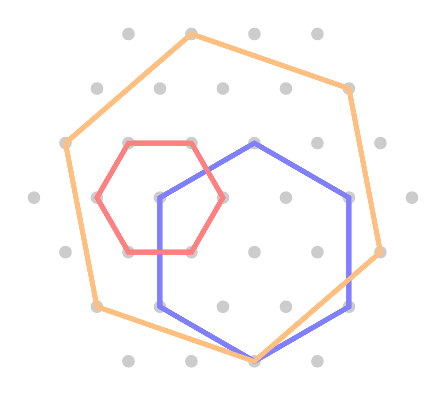
\begin{tikzpicture}[scale=0.8]
    \foreach \y/\n/\k in {1/4/0, 2/5/0, 3/6/0, 4/7/0, 5/6/1, 6/5/2, 7/4/3} {
      \foreach \x in {1,...,\n} {
        \fill[gray!40] ({\x - \y/2 + \k}, {sqrt(3)/2 * \y}) circle (0.1);
      }
      \draw[ultra thick, blue!50] (2.5, {sqrt(3)/2 * 1})--(1, {sqrt(3)/2 * 2})--(1, {sqrt(3)/2 * 4})--(2.5, {sqrt(3)/2 * 5})--(4, {sqrt(3)/2 * 4})--(4, {sqrt(3)/2 * 2})--cycle;
      \draw[ultra thick, red!50] (0.5, {sqrt(3)/2 * 3})--(0, {sqrt(3)/2 * 4})--(0.5, {sqrt(3)/2 * 5})--(1.5, {sqrt(3)/2 * 5})--(2, {sqrt(3)/2 * 4})--(1.5, {sqrt(3)/2 * 3})--cycle;
      % \draw[ultra thick, orange!50] (1.5, {sqrt(3)/2 * 7})--(3.5, {sqrt(3)/2 * 7})--(4.5, {sqrt(3)/2 * 5})--(3.5, {sqrt(3)/2 * 3})--(1.5, {sqrt(3)/2 * 3})--(0.5, {sqrt(3)/2 * 5})--cycle;
      \draw[ultra thick, orange!50] (1.5, {sqrt(3)/2 * 7})--(4, {sqrt(3)/2 * 6})--(4.5, {sqrt(3)/2 * 3})--(2.5, {sqrt(3)/2 * 1})--(0, {sqrt(3)/2 * 2})--(-0.5, {sqrt(3)/2 * 5})--cycle;
    }
  \end{tikzpicture}
  \caption{
    An illustration of three triangles on a triangular grid, three squares on
    a square grid, and three hexagons on a centered hexagonal grid.
  }
\end{figure}
\begin{question}
  Is there a combinatorial explanation for why these numbers relate to
  4-dimensional polytopes?
\end{question}

\begin{related}
  \item Can this be generalized to arbitrary regular $n$-gons in hyperbolic
    space?
  \item How many triangles are on the ``centered triangular number'' grid?

\end{related}
\begin{references}
  \item Problem 21.
  \item \url{https://en.wikipedia.org/wiki/Order-4_pentagonal_tiling}
\end{references}
\end{document}
